\documentclass{article}
\usepackage[utf8]{inputenc}
\usepackage[T1]{fontenc}
\usepackage{amsmath}
\usepackage{amsfonts}
\usepackage{amssymb}
\usepackage{amsthm}
\usepackage[many]{tcolorbox}

\usepackage{tikz}
\usetikzlibrary{positioning, fit, shapes}
\usetikzlibrary{shapes,decorations,arrows,positioning}
\tikzstyle{vertex}=[circle, draw, fill=blue!20]
\tikzstyle{set}=[rectangle, rounded corners, draw=black, dashed, inner sep=10pt, label=below:#1]
\tikzstyle{wire}=[thin]
\tikzstyle{cable}=[thick, red, ->, >=stealth]
\tikzstyle{legend} = [rectangle, rounded corners, fill=gray!10, minimum width=2cm, draw=black, align=left]

\usepackage[letterpaper, total={6in, 8in}]{geometry}


\title{MAT2719 -- notes de cours détaillées}
\date{Selon le cours d'Alexander Fribergh, Hiver 2024}
\author{Laurier Lavoie-Giasson, avec l'aide de ChatGPT 4}

\newtheoremstyle{pasdepoint}
  {\topsep}{\topsep}%
  {}{}%
  {\bfseries}{\vspace*{0.05in}\\}%
  {0pt}{}%
\theoremstyle{pasdepoint}
\newtheorem{definition}{Définition}
\tcolorboxenvironment{definition}{
    rounded corners,
    colback=yellow!5,
    before skip=0.2in,
    after skip=0.2in
}
\newtheoremstyle{break}
  {\topsep}{\topsep}%
  {}{}%
  {\bfseries}{}%
  {\newline}{}%
\theoremstyle{break}
\newtheorem{example}{Exemple}
\tcolorboxenvironment{example}{
    rounded corners,
    colback=blue!5,
    before skip=0.2in,
    after skip=0.2in
}

\theoremstyle{pasdepoint}
\newtheorem*{pourquoi}{Pourquoi ?}
\tcolorboxenvironment{pourquoi}{
    rounded corners,
    colback=yellow!10,
    before skip=0.2in,
    after skip=0.2in
}

\newtheorem*{remark}{Remarque}
\tcolorboxenvironment{remark}{
    rounded corners,
    colback=green!15,
    before skip=0.2in,
    after skip=0.2in
}

\newtheorem*{notation}{Notation}
\tcolorboxenvironment{notation}{
    rounded corners,
    colback=orange!20,
    before skip=0.2in,
    after skip=0.2in
}

\newtheorem*{prop}{Proposition}
\tcolorboxenvironment{prop}{
    rounded corners,
    colback=yellow!20,
    before skip=0.2in,
    after skip=0.2in
}
\begin{document}

\begin{titlepage}
    \maketitle
\end{titlepage}

\section{Définitions préalables}

\begin{definition}[Graphe]
    Un \textbf{graphe} $G$ est une paire ordonnée $G = (V, E)$ composée de :
    \begin{itemize}
        \item Un ensemble $V$ de \textit{sommet}, qui représente les points du graphe.
        \item Un ensemble $E$ d'\textit{arêtes}, qui sont des paires non ordonnées de sommets. Les arêtes relient les sommets entre eux.
    \end{itemize}
\end{definition}

En d'autres termes, un graphe est une structure de données utilisée pour modéliser un ensemble de relations entre des paires d'objets. Chaque sommet dans le graphe représente un objet, et chaque arête représente une relation entre deux objets.

    
\begin{example}[Graphe]
    \begin{tikzpicture}
        % Les nœuds
        \node (A) at (0,0) {A};
        \node (B) at (2,0) {B};
        \node (C) at (1,-1.5) {C};
        \node (D) at (3,-1.5) {D};
        \node (E) at (4.5,0) {E};

        % Les arêtes
        \draw (A) -- (B);
        \draw (B) -- (C);
        \draw (C) -- (A);
        \draw (C) -- (D);
        \draw (D) -- (E);
    \end{tikzpicture}

    Ici, $V = \{A, B, C, D, E\}$ et $E = \{(A, B), (B, C), (C, A), (C, D), (D, E)\}$.
\end{example}

Les graphes sont largement utilisés dans divers domaines pour modéliser et résoudre des problèmes complexes. En informatique, ils servent à représenter des réseaux sociaux, des itinéraires de navigation, des structures de données, et bien plus encore. Dans le domaine des transports, les graphes sont utilisés pour optimiser les itinéraires, la logistique et la gestion du trafic. En biologie, ils aident à modéliser les interactions entre protéines dans les réseaux de régulation génétique. En mathématiques, les graphes sont un outil essentiel pour la théorie des graphes, tandis qu'en chimie, ils sont utilisés pour représenter des molécules. En résumé, les graphes sont une structure de données polyvalente avec de nombreuses applications pratiques.

\begin{definition}[Chaîne de Markov]
    Une \textbf{chaîne de Markov}, notée $(X_n)_{n \geq 0}$, est un type spécifique de processus stochastique discret satisfaisant la propriété de Markov, qui stipule que, donné l'état présent, les états futurs sont indépendants des états passés. Formellement, pour tous les états $i$ et $j$ et tout $n \geq 0$, on a :
    \[
    P(Z_{n+1} = j | Z_n = i, Z_{n-1} = i_{n-1}, \ldots, Z_0 = i_0) = P(Z_{n+1} = j | Z_n = i)
    \]
\end{definition}

\begin{pourquoi}[Chaîne de Markov]
    Un lecteur n'ayant pas de connaissances approfondies des processus stochastiques pourrait se demander l'intérêt d'étudier les chaînes de Markov dans le contexte des marches et graphes aléatoires.

    On verra plus tard qu'une marche aléatoire \((X_n)_{n\in\mathbb{N}}\) sur un graphe \(G\) est essentiellement une chaîne de Markov, mais plus précisément dont les états possibles correspondent exactement aux noeuds de \(G\), et dont les probabilités de transition correspondent aux probabilités de \guillemotleft passage\guillemotright\ ou de \guillemotleft transition\guillemotright\ associées aux arêtes de \(G\).

    Il est cependant important de ne pas confondre le concept de chaîne de Markov avec celui d'une marche aléatoire; même si une chaîne de Markov peut souvent être représentée à l'aide d'un graphe, ce ne sont pas toutes les chaînes de Markov qui sont des marches aléatoires sur des graphes.
    
    Dans le cas général de la chaîne de Markov, le graphe utilisé pour représenter les états possibles de la chaîne et les probabilités de transition ne représente pas nécessairement un graphe précis -- il permet simplement une représentation claire et concise de la distribution de probabilités sous-jacente au processus stochastique en question.
\end{pourquoi}

\pagebreak \section{Marche aléatoire}

\begin{definition}[Marche aléatoire sur un graphe]
    Une \textbf{marche aléatoire} sur un graphe \(G = (V, E)\) est une séquence de variables aléatoires \((X_n)_{n\in\mathbb{N}}\) où chaque \(X_n\) représente la position d'un marcheur sur les sommets du graphe à l'étape \(n\). La marche est définie par les conditions suivantes :
    \begin{itemize}
        \item \(X_0\) est le sommet de départ, souvent choisi selon une distribution de probabilité spécifique sur \(V\).
        \item Pour chaque étape \(n > 0\), la probabilité que le marcheur se déplace de l'état \(i\) à l'état \(j\) est donnée par \(P(X_{n+1} = y | X_n = x)\), pour tous \(x, y \in V\), où \(P\) est la matrice de probabilités de transition du graphe.
        %\item La marche est dite \textit{réversible} si elle satisfait la condition de réversibilité: pour tous \(i, j \in V\), \(\pi(i)P(i, j) = \pi(j)P(j, i)\), où \(\pi\) est une distribution stationnaire associée à la marche.
    \end{itemize}
\end{definition}

Pour être répétitif: tel qu'indiqué dans la section précédente, une marche aléatoire discrète est généralement considérée comme un exemple classique de chaîne de Markov. Dans une marche aléatoire discrète, l'état futur (c'est-à-dire le prochain sommet visité dans le graphe) dépend uniquement de l'état actuel et pas des états précédents. Cette caractéristique satisfait la propriété fondamentale des chaînes de Markov, où la probabilité de transition vers l'état suivant ne dépend que de l'état actuel.

En termes simples, dans une marche aléatoire discrète sur un graphe, lorsqu'un individu se déplace d'un sommet à un autre, son choix du prochain sommet à visiter dépend uniquement de sa position actuelle et des probabilités de transition associées à cette position, et non de la manière dont il est arrivé à ce sommet. Cette indépendance par rapport à l'historique du chemin parcouru est exactement ce qui définit une chaîne de Markov.

\begin{notation}[Probabilité de transition dans une marche aléatoire]
    Considérons une marche aléatoire \( (X_n)_{n \in \mathbb{N}} \) sur un graphe. On définira la probabilité de transition \( p(x, y) \) d'un sommet \( x \) à un sommet \( y \) comme la probabilité que la marche se déplace de \( x \) à \( y \) en une seule étape. Formellement, pour deux sommets \( x \) et \( y \) du graphe,

    \[
    p(x, y) = P(X_{n+1} = y | X_n = x) = P(X_1 = y | X_0 = x)\text{ (par la propriété de Markov)}
    \]

    où \( P(X_{n+1} = y | X_n = x) \) est la probabilité conditionnelle que le prochain état de la marche soit \( y \), étant donné que l'état actuel est \( x \).
\end{notation}

\begin{remark}[lien entre marche aléatoire sur un graphe et sur la droite des entiers]
    Une \textbf{marche aléatoire sur un graphe} et une \textbf{marche aléatoire sur la droite des entiers} (\(\mathbb{Z}\)) sont deux exemples de processus stochastiques, en particulier des chaînes de Markov, mais avec des structures sous-jacentes différentes.

    \begin{itemize}
        \item Dans une \textbf{marche aléatoire sur un graphe}, chaque sommet représente un état et les arêtes définissent les transitions possibles entre les états. La probabilité de transition d'un sommet à un autre est définie par la matrice de probabilités de transition du graphe.
        \item Dans une \textbf{marche aléatoire sur \(\mathbb{Z}\)}, les états sont les entiers et les transitions se font typiquement d'un entier à son voisin immédiat (par exemple, de \(n\) à \(n+1\) ou \(n-1\)). La simplicité de la structure de \(\mathbb{Z}\) conduit souvent à des règles de transition plus simples.
    \end{itemize}

    Une \textbf{marche aléatoire sur} \(\mathbb{Z}\) peut être considérée dans le cadre plus général d'une marche aléatoire sur un graphe. Pour ce faire, conceptualisons \(\mathbb{Z}\) comme un graphe \(G = (V, E)\) où:
    \begin{itemize}
        \item L'ensemble des sommets \(V\) correspond à l'ensemble \(\mathbb{Z}\) des entiers.
        \item L'ensemble des arêtes \(E\) ainsi que la matrice de transition \(\mathbb{P}\) définit les transitions possibles entre les entiers.
    \end{itemize}

    Dans cette interprétation, une \textit{marche aléatoire sur} \(\mathbb{Z}\) est une marche sur le graphe \(G\), où la probabilité de transition de l'état \(i\) à l'état \(j\) (c'est-à-dire de l'entier \(i\) à l'entier \(j\)) est déterminée par une matrice de probabilités ou une règle spécifique. Cette approche permet une plus grande flexibilité dans la définition des transitions et peut inclure des marches avec des sauts plus longs ou des règles de transition complexes.
\end{remark}

\begin{definition}[Temps d'atteinte]
    Considérons un graphe \( G = (V, E) \) et un sous-ensemble \( U \subseteq V \). Soit \( W = V \setminus U \) et \( s \in U \).\\

    Le \textbf{temps d'atteinte} \( T_W \) pour un ensemble \( W \) est le premier instant \( n \geq 0 \) où la marche aléatoire \( (X_n)_{n\in\mathbb{N}} \) atteint un sommet dans \( W \). Formellement, 
    \[
    T_W = \min\{n \geq 0 : X_n \in W\}
    \]

    Le \textbf{temps d'atteinte strictement positif} \(T_W^+\) pour un ensemble \( W \) est le premier instant \( n > 0 \) où la marche aléatoire \( (X_n)_{n\in\mathbb{N}} \) atteint un sommet dans \( W \). Formellement,
    \[
    T_W^+ = \min\{n > 0 : X_n \in W\}
    \]
\end{definition}

\begin{definition}[Transience et Récurrence]
    Soit une marche aléatoire \( (X_n)_{n \in \mathbb{N}} \) sur un graphe \( G = (V, E) \) et soit \( x \in V \) un sommet du graphe. 
    
    \begin{itemize}
        \item \textbf{Récurrence :} Le sommet \( x \) est dit \textit{récurrent} si la probabilité qu'il soit revisité est de 1, c'est-à-dire si la probabilité que la marche, ayant commencé en \( x \), retourne à \( x \) en un temps fini est de 1. Formellement, \( x \) est récurrent si
        \[
        P_x[T_x^+ < \infty] = 1
        \]
        où \( T_x^+ \) est le temps de frappe strictement positif de \( x \), c'est-à-dire le premier instant \( n > 0 \) tel que \( X_n = x \).
    
        \item \textbf{Transience :} Le sommet \( x \) est dit \textit{transient} si la probabilité qu'il soit revisité est inférieure à 1. Autrement dit, \( x \) est transient si la probabilité que la marche ne retourne jamais à \( x \) après l'avoir quitté est non nulle. Formellement, \( x \) est transient si
        \[
        P_x[T_x^+ = \infty] > 0
        \]
        ou, de manière équivalente, si \( P_x[T_x^+ < \infty] < 1 \).
    \end{itemize}
\end{definition}

\section{Réversibilité d'une marche aléatoire}

\begin{definition}[Marche aléatoire réversible]
    Considérons une \textbf{marche aléatoire réversible} définie sur un graphe $G = (V, E)$, où $(X_n)_{n \in \mathbb{N}}$ représente une chaîne de Markov sur les sommets du graphe. Une telle marche est dite réversible par rapport à une distribution $\pi : V \rightarrow (0, +\infty)$ si elle satisfait la condition de réversibilité suivante :

    \[
    \pi(x)p(x, y) = \pi(y)p(y, x) \quad \text{pour tous les sommets } x, y \in V
    \]

    où $p(x, y)$ représente la probabilité de transition de l'état $x$ à l'état $y$.

\end{definition}

Cette relation signifie que pour tout couple de sommets $x$ et $y$, le produit de la probabilité de se déplacer de $x$ à $y$ et de la mesure stationnaire $\pi$ en $x$ est égal au produit de la probabilité de se déplacer de $y$ à $x$ et de la mesure stationnaire $\pi$ en $y$.

La réversibilité d'une marche aléatoire est une propriété importante qui implique que, dans un état d'équilibre, le processus se comporte de manière identique dans le temps, que l'on observe son évolution en avant ou en arrière. Dans le cadre des chaînes de Markov et des marches aléatoires sur des graphes, la réversibilité peut offrir des indices significatifs sur la structure du graphe et sur la dynamique du processus stochastique.
\begin{definition}[Conductance]
    La \textbf{conductance} entre deux sommets \(x\) et \(y\) dans un graphe \(G = (V, E)\), dans le contexte d'une marche aléatoire réversible, est définie par \(C(x, y) = \pi(x)p(x, y)\), où :
    \begin{itemize}
        \item \(\pi : V \rightarrow (0, +\infty)\) est une distribution sur les sommets du graphe, souvent interprétée comme une mesure stationnaire ou une distribution d'équilibre.
        \item \(p(x, y)\) est la probabilité de transition de l'état \(x\) à l'état \(y\).
    \end{itemize}

    La conductance mesure la "facilité" ou la "capacité" avec laquelle la marche peut se déplacer de \(x\) à \(y\), en tenant compte de la distribution \(\pi\). Dans le cadre d'une marche aléatoire réversible, où \(\pi(x)p(x, y) = \pi(y)p(y, x)\) pour tous les sommets \(x, y \in V\), la conductance satisfait la propriété de symétrie \(C(x, y) = C(y, x)\). Cette symétrie reflète la nature réversible de la marche, où la probabilité de transition dans un sens est équilibrée par la probabilité de transition dans le sens inverse, pondérée par la mesure stationnaire.

    La notion de conductance est cruciale dans l'analyse des propriétés de mélange et de diffusion des marches aléatoires sur des graphes, en particulier dans le contexte des chaînes de Markov réversibles.
\end{definition}

La distribution \(\pi : V \rightarrow (0, +\infty)\) dans une marche aléatoire réversible est souvent appelée \textbf{distribution d'équilibre} ou \textbf{mesure stationnaire}. Cette distribution est caractérisée par le fait qu'elle ne change pas au fil du temps lorsque la chaîne est observée. En d'autres termes, si la marche aléatoire commence avec la distribution \(\pi\), elle maintiendra cette même distribution à chaque étape subséquente.\\

L'équilibre est atteint lorsque, pour chaque sommet \(x\), le taux total de probabilité "entrant" dans \(x\) est égal au taux total de probabilité "sortant" de \(x\). Formellement, cela signifie que pour tout \(x \in V\),
\[
\sum_{y \in V} \pi(y)p(y, x) = \pi(x) = \sum_{y \in V} \pi(x)p(x, y)
\]
Cette équation exprime le fait que la probabilité d'être en \(x\) est conservée à travers les transitions de la marche. 

La relation avec la conductance, définie par \(C(x, y) = \pi(x)p(x, y)\), est clé dans la compréhension de cet équilibre. La réversibilité, impliquant que \(C(x, y) = C(y, x)\), assure que pour chaque paire de sommets \(x, y\), la quantité de "flux" de probabilité de \(x\) à \(y\) est équilibrée par le flux de \(y\) à \(x\). Cela crée un système en équilibre dynamique où, bien que les probabilités puissent circuler entre les états, la distribution globale reste invariante dans le temps.

\begin{notation}
    On utilise de manière interchangée \(\pi(x)\) et \(\pi_x\) afin de désigner la mesure \(\pi\) du sommet \(x\) du graphe.
    \[
        \pi_x = \pi(x)
    \]
\end{notation}
\begin{remark}
    Bien que l'on parle souvent des \((\pi_x)_{x \in V}\) en termes de probabilité, il est plus précis de les considérer comme une mesure. En mathématiques, une \textbf{mesure} est une fonction qui assigne un nombre non négatif (potentiellement infini) à certains sous-ensembles d'un ensemble donné, de manière à quantifier le "volume" ou la "taille" de ces sous-ensembles. En revanche, une \textbf{probabilité} est une mesure spéciale qui assigne un nombre réel entre 0 et 1 à des événements (sous-ensembles) dans un espace probabilisé, avec la propriété que la probabilité de l'espace entier est 1.
    
    Pour convertir une mesure en probabilité, on peut normaliser la mesure. Cela implique de diviser chaque valeur de la mesure par la somme totale des mesures sur tous les sous-ensembles considérés. Dans le contexte d'une chaîne de Markov, si \(\pi\) est initialement une mesure, on peut la transformer en une distribution de probabilité en normalisant chaque \(\pi_x\) tel que :
    \[
    \pi'_x = \frac{\pi_x}{\sum_{y \in V} \pi_y}
    \]
    où \(\pi'_x\) représente la probabilité normalisée d'être dans l'état \(x\). Après cette normalisation, la somme des \(\pi'_x\) pour tous les \(x \in V\) sera égale à 1, satisfaisant ainsi l'une des propriétés fondamentales d'une probabilité.
    \begin{notation}
        Sans perte de généralité, on pourra, selon le cas, faire un abus de notation et considérer que les \(\pi_x\) ont déjà été normalisés. Cela permettra d'alléger les explications dans plusieurs cas. \textbf{Il est cependant important de noter qu'une probabilité est une mesure, mais qu'une mesure n'est pas forcément une probabilité, et que les \(\pi_x\) sont des mesures avant tout, mais qui peuvent être normalisées afin d'obtenir une probabilité, tel que démontré ci-haut.}
    \end{notation}
\end{remark}
Dans ce contexte, le vecteur de probabilités \(\pi = (\pi_1, \pi_2, ..., \pi_k)\) pour une chaîne de Markov avec \(k\) états, représente la distribution stationnaire ou d'équilibre. Chaque composant \(\pi_i\) du vecteur indique la probabilité à long terme d'être dans l'état \(i\), après un grand nombre de transitions.

En pratique, cela signifie que si un instant \(N\) est choisi au hasard dans un futur lointain, la probabilité que la chaîne soit dans un état spécifique \(i\) à ce moment est \(\pi_i\). Cette probabilité est indépendante de l'état initial, à condition que la chaîne ait eu suffisamment de temps pour atteindre l'équilibre. La somme des composants de \(\pi\), c'est-à-dire \(\sum_{i=1}^{k} \pi_i\), est égale à 1, ce qui confirme que la chaîne doit se trouver dans l'un des états à tout moment donné. La constance de cette distribution au fil du temps illustre l'état d'équilibre de la chaîne de Markov, où la dynamique des transitions entre états ne modifie pas la distribution globale de probabilité, malgré le mouvement continu entre les différents états du système.

\begin{notation}
    Considérons un graphe \( G = (V, E) \). Pour deux sommets \( x, y \in V \), \(y \sim x\) indique que \(y\) est un voisin de \(x\).
    
    On utilisera souvent
    \[
        \sum_{y \sim x}\cdot
    \]
    afin de désigner une somme sur tous les \(y\) qui sont voisins de \(x\). Cette notation est utilisée pour désigner des opérations qui s'appliquent ou se réfèrent spécifiquement aux voisins de \( x \) dans le graphe.

    \begin{remark}
        Dès qu'une conductance apparaît comme coefficient dans une somme sur $y \sim x$, on a automatiquement l'égalité suivante:
        \[\sum_{y \sim x}c(x,y)\cdot = \sum_{y \in V}c(x,y)\cdot\]
        Car deux sommets qui de sont pas reliés par une arête ont une conductance équivalente à 0.
    \end{remark}
\end{notation}

\begin{prop}
    Pour une chaîne de Markov, la mesure stationnaire \(\pi(x)\) peut être dérivée des conductances \(c(x, y) = \pi(x)p(x, y)\) par le raisonnement suivant :
\[
\pi(x) = \sum_{y \sim x} c(x, y) = \sum_{y \sim x} \pi(x)p(x, y) = \pi(x) \sum_{y \sim x} p(x, y) = \pi(x)
\]
car \(\sum_{y \sim x} p(x, y) = 1\).\\

Ensuite, la probabilité de transition \(p(x, y)\) peut être exprimée comme:
\[
p(x, y) = \frac{c(x, y)}{\sum_{y \sim x} c(x, y)}
\]
\end{prop}

\begin{remark}
    Dans le cas d'une marche aléatoire réversible sur un graphe \( G = (V, E) \), considérons un cycle formé par une séquence de sommets \( x_1, \ldots, x_n \) tels que chaque \( x_i \) est voisin de \( x_{i+1} \) (c'est-à-dire \( x_i \sim x_{i+1} \)) et \( x_n = x_1 \). 

    La propriété de réversibilité d'une marche aléatoire implique que le produit des probabilités de transition le long du cycle est le même dans les deux sens. Formellement, cela signifie que:
    \[
    \prod_{i=1}^{n}p(x_i, x_{i+1}) = \prod_{i=1}^{n}p(x_{n+1-i}, x_{n-i})
    \]
    où \( p(x, y) \) est la probabilité de transition de l'état \( x \) à l'état \( y \), et par convention, \( x_{n+1} = x_1 \).

    Cette égalité découle de la propriété de réversibilité, qui stipule que \( p(x, y)\pi(x) = p(y, x)\pi(y) \) pour tous les sommets \( x, y \) dans \( V \). Elle met en évidence le fait qu'une marche réversible sur un cycle conserve le même "poids" de probabilité dans chaque direction du cycle.
\end{remark}

\begin{definition}[Fonction Harmonique]
    Une fonction \(f\) est dite \textbf{harmonique} sur un ensemble de sommets \(S\) d'un graphe si, pour chaque sommet \(v \in S\), la valeur de \(f\) en \(v\) est égale à la moyenne pondérée des valeurs de \(f\) sur les sommets voisins de \(v\). Formellement, pour un sommet \(v\) et ses voisins \(N(v)\),
    \[
    f(v) = \sum_{u \in N(v)} p(v, u) f(u)
    \]
    où \(p(v, u)\) est la probabilité de transition du sommet \(v\) au sommet \(u\). On dit que \(f\) est harmonique sur \(A \subset V\) si \(f\) est harmonique \(\forall x \in A\).
\end{definition}

\section{Applications des marches réversibles sur les circuits électriques}

On a déjà discutéans le contexte de circuits électriques

\section*{Principes du maximum, de l'unicité, de l'existence}

\begin{definition}[Principe du Maximum en Marches Aléatoires et Graphes]
    Soit \(G = (V, E)\) un graphe fini et \(f: V \rightarrow \mathbb{R}\) une fonction harmonique, c'est-à-dire \(f(x) = \sum_{y \sim x} p(x, y) f(y)\) pour tout \(x \in V\). Le principe du maximum affirme que le maximum et le minimum de \(f\) sont atteints aux sommets de la frontière de \(G\), là où \(x\) n'a pas de voisins extérieurs. Ce principe aide à déterminer les comportements extrêmes dans les marches aléatoires, tels que les probabilités maximales d'atteinte et les temps d'atteinte.
    \end{definition}
    

\pagebreak Soit \(A\) et \(Z\) deux sous-ensembles disjoints de \(G\). On appelle voltage (ou tension, ou potentiel) une fonction sur les sites de \(G\), qui est harmonique sur \((A \cup Z)^C\), constante sur \(A\) et constante sur \(Z\).

\begin{definition}[Voltage, Tension, ou Potentiel]
    Soit \(G = (V, E)\) un graphe, où \(V\) représente un ensemble de sommets et \(E\) représente un ensemble d'arêtes connectant ces sommets. Soient \(A\) et \(Z\) deux sous-ensembles disjoints de \(V\). Un \textbf{voltage} (ou tension, ou potentiel) est défini comme une fonction \(f: V \rightarrow \mathbb{R}\) qui satisfait les conditions suivantes :
    \begin{itemize}
        \item \(f\) est harmonique sur \((A \cup Z)^C\), c'est-à-dire pour tout sommet \(x \in (A \cup Z)^C\), la valeur de \(f\) en \(x\) est égale à la moyenne pondérée de \(f\) sur les voisins de \(x\).
        \item \(f\) est constante sur \(A\) et constante sur \(Z\), représentant typiquement des valeurs de potentiel fixées aux "bornes" ou aux "frontières" du graphe.
    \end{itemize}
    La différence de potentiel (voltage) entre deux points \(a \in A\) et \(z \in Z\) est alors donnée par la différence \(f(a) - f(z)\). Cette notion est fondamentale dans l'analyse des propriétés de transport et de diffusion sur les graphes, modélisant par exemple le comportement électrique dans les réseaux électriques ou les propriétés de circulation dans divers systèmes dynamiques.
\end{definition}
\begin{remark}
    Dans le contexte d'un système électrique comme celui d'une voiture, la différence de potentiel (voltage) entre la borne positive et la borne négative de la batterie est ce qui permet à l'électricité de circuler et au véhicule de fonctionner. Lors du survoltage d'une batterie, la différence de potentiel entre la borne positive et la borne négative de la voiture nécessitant un survoltage est augmentée par la connexion à une autre batterie avec un voltage supérieur. 

    Pour illustrer, si une voiture a besoin d'être survoltée parce que sa batterie a une tension trop faible, et une autre voiture (qui survolte) fournit un voltage supérieur via des câbles de démarrage, cela permet de rétablir le fonctionnement électrique de la première voiture. 

    Ce processus peut être modélisé par un graphe, où les sommets connectés à la borne positive de chaque batterie sont dans \(A\), ceux connectés à la borne négative sont dans \(Z\), et le flux d'électricité est représenté par le potentiel harmonique sur les autres sommets du graphe.

    \begin{example}
        Le graphe ci-dessous représente un modèle simplifié du circuit électrique d'une voiture avec une batterie faible.
        
        Les bornes "+" et "-" indiquent respectivement la borne positive et la borne négative de la batterie. La composante au milieu symbolise le circuit électrique de la voiture, incluant des composants tels que les phares, le démarreur et la radio. Dans ce modèle, la différence de potentiel entre les bornes "+" et "-" est insuffisante pour surmonter la résistance interne du circuit, ce qui empêche le démarrage de la voiture. Cette situation illustre un problème commun dans les véhicules avec des batteries déchargées ou en fin de vie.
        \begin{center}
            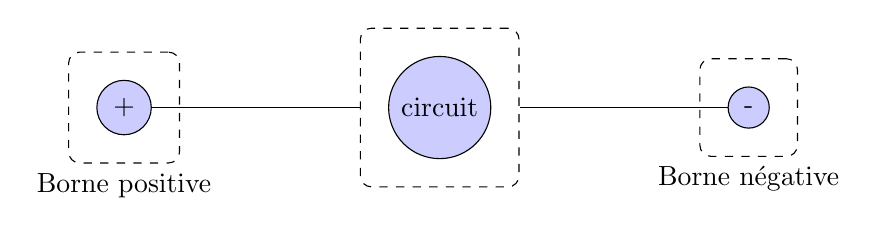
\begin{tikzpicture}[auto, node distance=3cm]
                % Noeuds
                \node[vertex] (plus) {+};
                \node[vertex, right=of plus] (A) {circuit};
                \node[vertex, right=of A] (minus) {-};
                \node[set, fit=(A)] (circuit) {};
                \draw[wire] (plus) -- (circuit);
                \draw[wire] (minus) -- (circuit);

                % Ensemble bornes
                \node[set=Borne positive, fit=(plus)] {};
                \node[set=Borne négative, fit=(minus)] {};
            \end{tikzpicture}
        \end{center}
            

        \bigskip % Ajoute un espace vertical pour la séparation
        
        Observons maintenant un second graphe, qui étend le modèle précédent en introduisant une solution au problème de la batterie faible: le survoltage. En ajoutant une batterie externe avec une charge suffisante, représentée par les bornes supplémentaires "+'" (borne positive de la batterie survoltée) et "-'" (borne négative de la batterie survoltée), nous augmentons artificiellement la différence de potentiel entre les bornes de la batterie faible. Les câbles de survoltage, illustrés par les arêtes reliant "+'" à "+" et "-'" à "-", permettent de transférer l'énergie de la batterie survoltée à la batterie faible. Ce processus augmente le potentiel disponible pour alimenter le circuit électrique de la voiture, permettant ainsi de surmonter la résistance du circuit et de démarrer le moteur. Cette approche est couramment utilisée pour démarrer des véhicules dont la batterie ne possède pas assez de charge pour initier le processus de démarrage par eux-mêmes.
        \begin{center}
            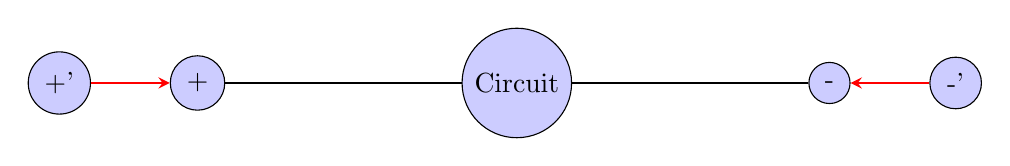
\begin{tikzpicture}[auto, node distance=3cm]
                % Noeuds
                \node[vertex] (plus) {+};
                \node[vertex, right=of plus] (A) {Circuit};
                \node[vertex, right=of A] (minus) {-};
            
                % Connexion de la batterie faible au circuit
                \draw[wire] (plus) -- (A);
                \draw[wire] (minus) -- (A);
            
                % Ajout des bornes de la batterie de survoltage
                \node[vertex, left=1cm of plus] (plusPrime) {+'};
                \node[vertex, right=1cm of minus] (minusPrime) {-'};
            
                % Câbles de survoltage
                \draw[cable] (plusPrime) -- (plus);
                \draw[cable] (minusPrime) -- (minus);
            \end{tikzpicture}
        \end{center}
    \end{example}

\end{remark}

\end{document}